\documentclass[1p]{elsarticle_modified}
%\bibliographystyle{elsarticle-num}

%\usepackage[colorlinks]{hyperref}
%\usepackage{abbrmath_seonhwa} %\Abb, \Ascr, \Acal ,\Abf, \Afrak
\usepackage{amsfonts}
\usepackage{amssymb}
\usepackage{amsmath}
\usepackage{amsthm}
\usepackage{scalefnt}
\usepackage{amsbsy}
\usepackage{kotex}
\usepackage{caption}
\usepackage{subfig}
\usepackage{color}
\usepackage{graphicx}
\usepackage{xcolor} %% white, black, red, green, blue, cyan, magenta, yellow
\usepackage{float}
\usepackage{setspace}
\usepackage{hyperref}

\usepackage{tikz}
\usetikzlibrary{arrows}

\usepackage{multirow}
\usepackage{array} % fixed length table
\usepackage{hhline}

%%%%%%%%%%%%%%%%%%%%%
\makeatletter
\renewcommand*\env@matrix[1][\arraystretch]{%
	\edef\arraystretch{#1}%
	\hskip -\arraycolsep
	\let\@ifnextchar\new@ifnextchar
	\array{*\c@MaxMatrixCols c}}
\makeatother %https://tex.stackexchange.com/questions/14071/how-can-i-increase-the-line-spacing-in-a-matrix
%%%%%%%%%%%%%%%

\usepackage[normalem]{ulem}

\newcommand{\msout}[1]{\ifmmode\text{\sout{\ensuremath{#1}}}\else\sout{#1}\fi}
%SOURCE: \msout is \stkout macro in https://tex.stackexchange.com/questions/20609/strikeout-in-math-mode

\newcommand{\cancel}[1]{
	\ifmmode
	{\color{red}\msout{#1}}
	\else
	{\color{red}\sout{#1}}
	\fi
}

\newcommand{\add}[1]{
	{\color{blue}\uwave{#1}}
}

\newcommand{\replace}[2]{
	\ifmmode
	{\color{red}\msout{#1}}{\color{blue}\uwave{#2}}
	\else
	{\color{red}\sout{#1}}{\color{blue}\uwave{#2}}
	\fi
}

\newcommand{\Sol}{\mathcal{S}} %segment
\newcommand{\D}{D} %diagram
\newcommand{\A}{\mathcal{A}} %arc


%%%%%%%%%%%%%%%%%%%%%%%%%%%%%5 test

\def\sl{\operatorname{\textup{SL}}(2,\Cbb)}
\def\psl{\operatorname{\textup{PSL}}(2,\Cbb)}
\def\quan{\mkern 1mu \triangleright \mkern 1mu}

\theoremstyle{definition}
\newtheorem{thm}{Theorem}[section]
\newtheorem{prop}[thm]{Proposition}
\newtheorem{lem}[thm]{Lemma}
\newtheorem{ques}[thm]{Question}
\newtheorem{cor}[thm]{Corollary}
\newtheorem{defn}[thm]{Definition}
\newtheorem{exam}[thm]{Example}
\newtheorem{rmk}[thm]{Remark}
\newtheorem{alg}[thm]{Algorithm}

\newcommand{\I}{\sqrt{-1}}
\begin{document}

%\begin{frontmatter}
%
%\title{Boundary parabolic representations of knots up to 8 crossings}
%
%%% Group authors per affiliation:
%\author{Yunhi Cho} 
%\address{Department of Mathematics, University of Seoul, Seoul, Korea}
%\ead{yhcho@uos.ac.kr}
%
%
%\author{Seonhwa Kim} %\fnref{s_kim}}
%\address{Center for Geometry and Physics, Institute for Basic Science, Pohang, 37673, Korea}
%\ead{ryeona17@ibs.re.kr}
%
%\author{Hyuk Kim}
%\address{Department of Mathematical Sciences, Seoul National University, Seoul 08826, Korea}
%\ead{hyukkim@snu.ac.kr}
%
%\author{Seokbeom Yoon}
%\address{Department of Mathematical Sciences, Seoul National University, Seoul, 08826,  Korea}
%\ead{sbyoon15@snu.ac.kr}
%
%\begin{abstract}
%We find all boundary parabolic representation of knots up to 8 crossings.
%
%\end{abstract}
%\begin{keyword}
%    \MSC[2010] 57M25 
%\end{keyword}
%
%\end{frontmatter}

%\linenumbers
%\tableofcontents
%
\newcommand\colored[1]{\textcolor{white}{\rule[-0.35ex]{0.8em}{1.4ex}}\kern-0.8em\color{red} #1}%
%\newcommand\colored[1]{\textcolor{white}{ #1}\kern-2.17ex	\textcolor{white}{ #1}\kern-1.81ex	\textcolor{white}{ #1}\kern-2.15ex\color{red}#1	}

{\Large $\underline{12n_{0273}~(K12n_{0273})}$}

\setlength{\tabcolsep}{10pt}
\renewcommand{\arraystretch}{1.6}
\vspace{1cm}\begin{tabular}{m{100pt}>{\centering\arraybackslash}m{274pt}}
\multirow{5}{120pt}{
	\centering
	\includegraphics[width=112pt]{../../../GIT/diagram.site/Diagrams/png/2362_12n_0273.png}\\
\ \ \ A knot diagram\footnotemark}&
\allowdisplaybreaks
\textbf{Linearized knot diagam} \\
\cline{2-2}
 &
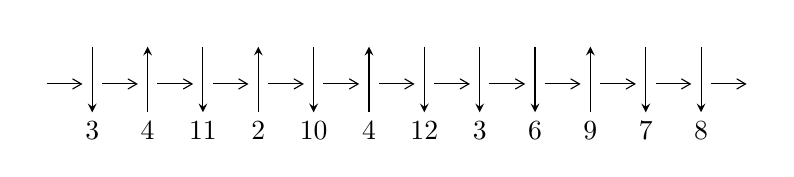
\begin{tikzpicture}[x=20pt, y=17pt]
	% nodes
	\node (C0) at (0, 0) {};
	\node (C1) at (1, 0) {};
	\node (C1U) at (1, +1) {};
	\node (C1D) at (1, -1) {3};

	\node (C2) at (2, 0) {};
	\node (C2U) at (2, +1) {};
	\node (C2D) at (2, -1) {4};

	\node (C3) at (3, 0) {};
	\node (C3U) at (3, +1) {};
	\node (C3D) at (3, -1) {11};

	\node (C4) at (4, 0) {};
	\node (C4U) at (4, +1) {};
	\node (C4D) at (4, -1) {2};

	\node (C5) at (5, 0) {};
	\node (C5U) at (5, +1) {};
	\node (C5D) at (5, -1) {10};

	\node (C6) at (6, 0) {};
	\node (C6U) at (6, +1) {};
	\node (C6D) at (6, -1) {4};

	\node (C7) at (7, 0) {};
	\node (C7U) at (7, +1) {};
	\node (C7D) at (7, -1) {12};

	\node (C8) at (8, 0) {};
	\node (C8U) at (8, +1) {};
	\node (C8D) at (8, -1) {3};

	\node (C9) at (9, 0) {};
	\node (C9U) at (9, +1) {};
	\node (C9D) at (9, -1) {6};

	\node (C10) at (10, 0) {};
	\node (C10U) at (10, +1) {};
	\node (C10D) at (10, -1) {9};

	\node (C11) at (11, 0) {};
	\node (C11U) at (11, +1) {};
	\node (C11D) at (11, -1) {7};

	\node (C12) at (12, 0) {};
	\node (C12U) at (12, +1) {};
	\node (C12D) at (12, -1) {8};
	\node (C13) at (13, 0) {};

	% arrows
	\draw[->,>={angle 60}]
	(C0) edge (C1) (C1) edge (C2) (C2) edge (C3) (C3) edge (C4) (C4) edge (C5) (C5) edge (C6) (C6) edge (C7) (C7) edge (C8) (C8) edge (C9) (C9) edge (C10) (C10) edge (C11) (C11) edge (C12) (C12) edge (C13) ;	\draw[->,>=stealth]
	(C1U) edge (C1D) (C2D) edge (C2U) (C3U) edge (C3D) (C4D) edge (C4U) (C5U) edge (C5D) (C6D) edge (C6U) (C7U) edge (C7D) (C8U) edge (C8D) (C9U) edge (C9D) (C10D) edge (C10U) (C11U) edge (C11D) (C12U) edge (C12D) ;
	\end{tikzpicture} \\
\hhline{~~} \\& 
\textbf{Solving Sequence} \\ \cline{2-2} 
 &
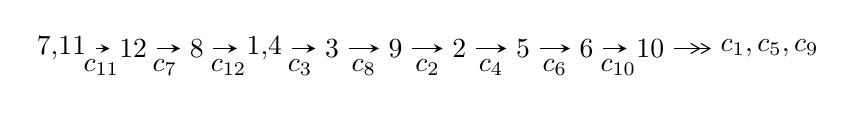
\begin{tikzpicture}[x=23pt, y=7pt]
	% node
	\node (A0) at (-1/8, 0) {7,11};
	\node (A1) at (1, 0) {12};
	\node (A2) at (2, 0) {8};
	\node (A3) at (49/16, 0) {1,4};
	\node (A4) at (33/8, 0) {3};
	\node (A5) at (41/8, 0) {9};
	\node (A6) at (49/8, 0) {2};
	\node (A7) at (57/8, 0) {5};
	\node (A8) at (65/8, 0) {6};
	\node (A9) at (73/8, 0) {10};
	\node (C1) at (1/2, -1) {$c_{11}$};
	\node (C2) at (3/2, -1) {$c_{7}$};
	\node (C3) at (5/2, -1) {$c_{12}$};
	\node (C4) at (29/8, -1) {$c_{3}$};
	\node (C5) at (37/8, -1) {$c_{8}$};
	\node (C6) at (45/8, -1) {$c_{2}$};
	\node (C7) at (53/8, -1) {$c_{4}$};
	\node (C8) at (61/8, -1) {$c_{6}$};
	\node (C9) at (69/8, -1) {$c_{10}$};
	\node (A10) at (11, 0) {$c_{1},c_{5},c_{9}$};

	% edge
	\draw[->,>=stealth]	
	(A0) edge (A1) (A1) edge (A2) (A2) edge (A3) (A3) edge (A4) (A4) edge (A5) (A5) edge (A6) (A6) edge (A7) (A7) edge (A8) (A8) edge (A9) ;
	\draw[->>,>={angle 60}]	
	(A9) edge (A10);
\end{tikzpicture} \\ 

\end{tabular} \\

\footnotetext{
The image of knot diagram is generated by the software ``\textbf{Draw programme}" developed by Andrew Bartholomew(\url{http://www.layer8.co.uk/maths/draw/index.htm\#Running-draw}), where we modified some parts for our purpose(\url{https://github.com/CATsTAILs/LinksPainter}).
}\phantom \\ \newline 
\centering \textbf{Ideals for irreducible components\footnotemark of $X_{\text{par}}$} 
 
\begin{align*}
I^u_{1}&=\langle 
-5 u^7-12 u^6+30 u^5+104 u^4+50 u^3-36 u^2+4 b+4 u+12,\\
\phantom{I^u_{1}}&\phantom{= \langle  }6 u^7+15 u^6-36 u^5-130 u^4-62 u^3+54 u^2+4 a-4 u-20,\\
\phantom{I^u_{1}}&\phantom{= \langle  }u^8+4 u^7-2 u^6-30 u^5-44 u^4-12 u^3+8 u^2-4 u-4\rangle \\
I^u_{2}&=\langle 
- a u+b+2 a- u+2,\;2 a^2- a u+2 a+u+3,\;u^2-2\rangle \\
I^u_{3}&=\langle 
u^2+2 b+2 a-4 u+2,\;4 u^2 a+2 a^2-12 a u- u^2+6 a+7 u-6,\;u^3-4 u^2+4 u-2\rangle \\
I^u_{4}&=\langle 
2 b+2 a+u+2,\;2 a^2+2 a u+2 a+u+3,\;u^2-2\rangle \\
\\
I^v_{1}&=\langle 
a,\;b^2- b+1,\;v+1\rangle \\
I^v_{2}&=\langle 
a,\;b+v-1,\;v^2- v+1\rangle \\
\end{align*}
\raggedright * 6 irreducible components of $\dim_{\mathbb{C}}=0$, with total 26 representations.\\
\footnotetext{All coefficients of polynomials are rational numbers. But the coefficients are sometimes approximated in decimal forms when there is not enough margin.}
\newpage
\renewcommand{\arraystretch}{1}
\centering \section*{I. $I^u_{1}= \langle -5 u^7-12 u^6+\cdots+4 b+12,\;6 u^7+15 u^6+\cdots+4 a-20,\;u^8+4 u^7+\cdots-4 u-4 \rangle$}
\flushleft \textbf{(i) Arc colorings}\\
\begin{tabular}{m{7pt} m{180pt} m{7pt} m{180pt} }
\flushright $a_{7}=$&$\begin{pmatrix}0\\u\end{pmatrix}$ \\
\flushright $a_{11}=$&$\begin{pmatrix}1\\0\end{pmatrix}$ \\
\flushright $a_{12}=$&$\begin{pmatrix}1\\u^2\end{pmatrix}$ \\
\flushright $a_{8}=$&$\begin{pmatrix}- u\\- u^3+u\end{pmatrix}$ \\
\flushright $a_{1}=$&$\begin{pmatrix}- u^2+1\\- u^4+2 u^2\end{pmatrix}$ \\
\flushright $a_{4}=$&$\begin{pmatrix}-\frac{3}{2} u^7-\frac{15}{4} u^6+\cdots+u+5\\\frac{5}{4} u^7+3 u^6+\cdots- u-3\end{pmatrix}$ \\
\flushright $a_{3}=$&$\begin{pmatrix}-\frac{1}{4} u^7-\frac{3}{4} u^6+\cdots-\frac{9}{2} u^2+2\\\frac{5}{4} u^7+3 u^6+\cdots- u-3\end{pmatrix}$ \\
\flushright $a_{9}=$&$\begin{pmatrix}-\frac{9}{4} u^7-\frac{23}{4} u^6+\cdots-\frac{25}{2} u^2+6\\\frac{3}{4} u^7+2 u^6-4 u^5-17 u^4-\frac{23}{2} u^3+4 u^2-2\end{pmatrix}$ \\
\flushright $a_{2}=$&$\begin{pmatrix}\frac{5}{4} u^7+\frac{11}{4} u^6+\cdots- u-2\\\frac{3}{4} u^7+2 u^6+\cdots- u-2\end{pmatrix}$ \\
\flushright $a_{5}=$&$\begin{pmatrix}- u^7-2 u^6+6 u^5+19 u^4+8 u^3-9 u^2+3\\- u^4+2 u^2\end{pmatrix}$ \\
\flushright $a_{6}=$&$\begin{pmatrix}3 u^7+\frac{31}{4} u^6+\cdots-2 u-9\\-\frac{3}{4} u^7-2 u^6+\cdots+u+2\end{pmatrix}$ \\
\flushright $a_{10}=$&$\begin{pmatrix}-\frac{1}{2} u^7-\frac{5}{4} u^6+\cdots-\frac{5}{2} u^2+2\\\frac{1}{4} u^7+u^6- u^5-8 u^4-\frac{13}{2} u^3+2 u^2-1\end{pmatrix}$\\&\end{tabular}
\flushleft \textbf{(ii) Obstruction class $= -1$}\\~\\
\flushleft \textbf{(iii) Cusp Shapes $= -2 u^7-4 u^6+13 u^5+35 u^4+8 u^3-6 u^2+18 u-2$}\\~\\
\newpage\renewcommand{\arraystretch}{1}
\flushleft \textbf{(iv) u-Polynomials at the component}\newline \\
\begin{tabular}{m{50pt}|m{274pt}}
Crossings & \hspace{64pt}u-Polynomials at each crossing \\
\hline $$\begin{aligned}c_{1}\end{aligned}$$&$\begin{aligned}
&u^8-4 u^7-142 u^6-1344 u^5+923 u^4-512 u^3+178 u^2-36 u+1
\end{aligned}$\\
\hline $$\begin{aligned}c_{2},c_{4},c_{10}\end{aligned}$$&$\begin{aligned}
&u^8-2 u^6+40 u^5-73 u^4+56 u^3-18 u^2+1
\end{aligned}$\\
\hline $$\begin{aligned}c_{3},c_{5},c_{9}\end{aligned}$$&$\begin{aligned}
&u^8-6 u^5- u^4-6 u^3-2 u^2-2 u-1
\end{aligned}$\\
\hline $$\begin{aligned}c_{6}\end{aligned}$$&$\begin{aligned}
&u^8-6 u^7+22 u^6-102 u^5+297 u^4-492 u^3+402 u^2-108 u-19
\end{aligned}$\\
\hline $$\begin{aligned}c_{7},c_{11},c_{12}\end{aligned}$$&$\begin{aligned}
&u^8+4 u^7-2 u^6-30 u^5-44 u^4-12 u^3+8 u^2-4 u-4
\end{aligned}$\\
\hline $$\begin{aligned}c_{8}\end{aligned}$$&$\begin{aligned}
&u^8-16 u^7+72 u^6-4 u^5-371 u^4-426 u^3+442 u^2+68 u-97
\end{aligned}$\\
\hline
\end{tabular}\\~\\
\newpage\renewcommand{\arraystretch}{1}
\flushleft \textbf{(v) Riley Polynomials at the component}\newline \\
\begin{tabular}{m{50pt}|m{274pt}}
Crossings & \hspace{64pt}Riley Polynomials at each crossing \\
\hline $$\begin{aligned}c_{1}\end{aligned}$$&$\begin{aligned}
&y^8-300 y^7+\cdots-940 y+1
\end{aligned}$\\
\hline $$\begin{aligned}c_{2},c_{4},c_{10}\end{aligned}$$&$\begin{aligned}
&y^8-4 y^7-142 y^6-1344 y^5+923 y^4-512 y^3+178 y^2-36 y+1
\end{aligned}$\\
\hline $$\begin{aligned}c_{3},c_{5},c_{9}\end{aligned}$$&$\begin{aligned}
&y^8-2 y^6-40 y^5-73 y^4-56 y^3-18 y^2+1
\end{aligned}$\\
\hline $$\begin{aligned}c_{6}\end{aligned}$$&$\begin{aligned}
&y^8+8 y^7+\cdots-26940 y+361
\end{aligned}$\\
\hline $$\begin{aligned}c_{7},c_{11},c_{12}\end{aligned}$$&$\begin{aligned}
&y^8-20 y^7+156 y^6-612 y^5+1208 y^4-1072 y^3+320 y^2-80 y+16
\end{aligned}$\\
\hline $$\begin{aligned}c_{8}\end{aligned}$$&$\begin{aligned}
&y^8-112 y^7+\cdots-90372 y+9409
\end{aligned}$\\
\hline
\end{tabular}\\~\\
\newpage\flushleft \textbf{(vi) Complex Volumes and Cusp Shapes}
$$\begin{array}{c|c|c}  
\text{Solutions to }I^u_{1}& \I (\text{vol} + \sqrt{-1}CS) & \text{Cusp shape}\\
 \hline 
\begin{aligned}
u &= -0.551137\phantom{ +0.000000I} \\
a &= \phantom{-}0.212410\phantom{ +0.000000I} \\
b &= \phantom{-}0.424769\phantom{ +0.000000I}\end{aligned}
 & -0.800674\phantom{ +0.000000I} & -12.5950\phantom{ +0.000000I} \\ \hline\begin{aligned}
u &= -1.44764 + 0.06689 I \\
a &= -0.812880 - 0.861044 I \\
b &= -0.292648 + 0.756441 I\end{aligned}
 & -4.25535 + 2.66770 I & -4.04426 - 2.00132 I \\ \hline\begin{aligned}
u &= -1.44764 - 0.06689 I \\
a &= -0.812880 + 0.861044 I \\
b &= -0.292648 - 0.756441 I\end{aligned}
 & -4.25535 - 2.66770 I & -4.04426 + 2.00132 I \\ \hline\begin{aligned}
u &= \phantom{-}0.377266 + 0.364501 I \\
a &= \phantom{-}1.01991 - 1.65688 I \\
b &= \phantom{-}0.110704 + 0.754072 I\end{aligned}
 & \phantom{-}1.63452 - 1.28115 I & \phantom{-}0.91619 + 5.71849 I \\ \hline\begin{aligned}
u &= \phantom{-}0.377266 - 0.364501 I \\
a &= \phantom{-}1.01991 + 1.65688 I \\
b &= \phantom{-}0.110704 - 0.754072 I\end{aligned}
 & \phantom{-}1.63452 + 1.28115 I & \phantom{-}0.91619 - 5.71849 I \\ \hline\begin{aligned}
u &= -2.04666 + 0.56570 I \\
a &= \phantom{-}0.01556 + 1.77149 I \\
b &= \phantom{-}0.98351 - 1.43901 I\end{aligned}
 & \phantom{-}13.6112 + 10.0113 I & -6.52481 - 3.89603 I \\ \hline\begin{aligned}
u &= -2.04666 - 0.56570 I \\
a &= \phantom{-}0.01556 - 1.77149 I \\
b &= \phantom{-}0.98351 + 1.43901 I\end{aligned}
 & \phantom{-}13.6112 - 10.0113 I & -6.52481 + 3.89603 I \\ \hline\begin{aligned}
u &= \phantom{-}2.78520\phantom{ +0.000000I} \\
a &= \phantom{-}1.34242\phantom{ +0.000000I} \\
b &= -2.02789\phantom{ +0.000000I}\end{aligned}
 & -11.3105\phantom{ +0.000000I} & -8.09900\phantom{ +0.000000I}\\
 \hline 
 \end{array}$$\newpage\newpage\renewcommand{\arraystretch}{1}
\centering \section*{II. $I^u_{2}= \langle - a u+b+2 a- u+2,\;2 a^2- a u+2 a+u+3,\;u^2-2 \rangle$}
\flushleft \textbf{(i) Arc colorings}\\
\begin{tabular}{m{7pt} m{180pt} m{7pt} m{180pt} }
\flushright $a_{7}=$&$\begin{pmatrix}0\\u\end{pmatrix}$ \\
\flushright $a_{11}=$&$\begin{pmatrix}1\\0\end{pmatrix}$ \\
\flushright $a_{12}=$&$\begin{pmatrix}1\\2\end{pmatrix}$ \\
\flushright $a_{8}=$&$\begin{pmatrix}- u\\- u\end{pmatrix}$ \\
\flushright $a_{1}=$&$\begin{pmatrix}-1\\0\end{pmatrix}$ \\
\flushright $a_{4}=$&$\begin{pmatrix}a\\a u-2 a+u-2\end{pmatrix}$ \\
\flushright $a_{3}=$&$\begin{pmatrix}a u- a+u-2\\a u-2 a+u-2\end{pmatrix}$ \\
\flushright $a_{9}=$&$\begin{pmatrix}- a-\frac{1}{2} u-2\\a u-2 a+u-1\end{pmatrix}$ \\
\flushright $a_{2}=$&$\begin{pmatrix}2 a u-3 a+\frac{3}{2} u-4\\a u-2 a+u-1\end{pmatrix}$ \\
\flushright $a_{5}=$&$\begin{pmatrix}1\\0\end{pmatrix}$ \\
\flushright $a_{6}=$&$\begin{pmatrix}a u- a+\frac{3}{2} u+1\\- a u+2 a- u+1\end{pmatrix}$ \\
\flushright $a_{10}=$&$\begin{pmatrix}a- u\\a u-2 a+u-2\end{pmatrix}$\\&\end{tabular}
\flushleft \textbf{(ii) Obstruction class $= 1$}\\~\\
\flushleft \textbf{(iii) Cusp Shapes $= -8 a u+16 a-8 u+4$}\\~\\
\newpage\renewcommand{\arraystretch}{1}
\flushleft \textbf{(iv) u-Polynomials at the component}\newline \\
\begin{tabular}{m{50pt}|m{274pt}}
Crossings & \hspace{64pt}u-Polynomials at each crossing \\
\hline $$\begin{aligned}c_{1},c_{3},c_{4}\\c_{9},c_{10}\end{aligned}$$&$\begin{aligned}
&(u^2- u+1)^2
\end{aligned}$\\
\hline $$\begin{aligned}c_{2},c_{5}\end{aligned}$$&$\begin{aligned}
&(u^2+u+1)^2
\end{aligned}$\\
\hline $$\begin{aligned}c_{6}\end{aligned}$$&$\begin{aligned}
&u^4+2 u^3+5 u^2+10 u+7
\end{aligned}$\\
\hline $$\begin{aligned}c_{7},c_{11},c_{12}\end{aligned}$$&$\begin{aligned}
&(u^2-2)^2
\end{aligned}$\\
\hline $$\begin{aligned}c_{8}\end{aligned}$$&$\begin{aligned}
&u^4-2 u^3+5 u^2-10 u+7
\end{aligned}$\\
\hline
\end{tabular}\\~\\
\newpage\renewcommand{\arraystretch}{1}
\flushleft \textbf{(v) Riley Polynomials at the component}\newline \\
\begin{tabular}{m{50pt}|m{274pt}}
Crossings & \hspace{64pt}Riley Polynomials at each crossing \\
\hline $$\begin{aligned}c_{1},c_{2},c_{3}\\c_{4},c_{5},c_{9}\\c_{10}\end{aligned}$$&$\begin{aligned}
&(y^2+y+1)^2
\end{aligned}$\\
\hline $$\begin{aligned}c_{6},c_{8}\end{aligned}$$&$\begin{aligned}
&y^4+6 y^3- y^2-30 y+49
\end{aligned}$\\
\hline $$\begin{aligned}c_{7},c_{11},c_{12}\end{aligned}$$&$\begin{aligned}
&(y-2)^4
\end{aligned}$\\
\hline
\end{tabular}\\~\\
\newpage\flushleft \textbf{(vi) Complex Volumes and Cusp Shapes}
$$\begin{array}{c|c|c}  
\text{Solutions to }I^u_{2}& \I (\text{vol} + \sqrt{-1}CS) & \text{Cusp shape}\\
 \hline 
\begin{aligned}
u &= \phantom{-}1.41421\phantom{ +0.000000I} \\
a &= -0.14645 + 1.47840 I \\
b &= -0.500000 - 0.866025 I\end{aligned}
 & -4.93480 - 4.05977 I & -8.00000 + 6.92820 I \\ \hline\begin{aligned}
u &= \phantom{-}1.41421\phantom{ +0.000000I} \\
a &= -0.14645 - 1.47840 I \\
b &= -0.500000 + 0.866025 I\end{aligned}
 & -4.93480 + 4.05977 I & -8.00000 - 6.92820 I \\ \hline\begin{aligned}
u &= -1.41421\phantom{ +0.000000I} \\
a &= -0.853553 + 0.253653 I \\
b &= -0.500000 - 0.866025 I\end{aligned}
 & -4.93480 - 4.05977 I & -8.00000 + 6.92820 I \\ \hline\begin{aligned}
u &= -1.41421\phantom{ +0.000000I} \\
a &= -0.853553 - 0.253653 I \\
b &= -0.500000 + 0.866025 I\end{aligned}
 & -4.93480 + 4.05977 I & -8.00000 - 6.92820 I\\
 \hline 
 \end{array}$$\newpage\newpage\renewcommand{\arraystretch}{1}
\centering \section*{III. $I^u_{3}= \langle u^2+2 b+2 a-4 u+2,\;4 u^2 a+2 a^2-12 a u- u^2+6 a+7 u-6,\;u^3-4 u^2+4 u-2 \rangle$}
\flushleft \textbf{(i) Arc colorings}\\
\begin{tabular}{m{7pt} m{180pt} m{7pt} m{180pt} }
\flushright $a_{7}=$&$\begin{pmatrix}0\\u\end{pmatrix}$ \\
\flushright $a_{11}=$&$\begin{pmatrix}1\\0\end{pmatrix}$ \\
\flushright $a_{12}=$&$\begin{pmatrix}1\\u^2\end{pmatrix}$ \\
\flushright $a_{8}=$&$\begin{pmatrix}- u\\-4 u^2+5 u-2\end{pmatrix}$ \\
\flushright $a_{1}=$&$\begin{pmatrix}- u^2+1\\-10 u^2+14 u-8\end{pmatrix}$ \\
\flushright $a_{4}=$&$\begin{pmatrix}a\\-\frac{1}{2} u^2- a+2 u-1\end{pmatrix}$ \\
\flushright $a_{3}=$&$\begin{pmatrix}-\frac{1}{2} u^2+2 u-1\\-\frac{1}{2} u^2- a+2 u-1\end{pmatrix}$ \\
\flushright $a_{9}=$&$\begin{pmatrix}a u+u^2- a-2 u+2\\- u^2 a+2 a u-\frac{3}{2} u^2- a+3 u-1\end{pmatrix}$ \\
\flushright $a_{2}=$&$\begin{pmatrix}\frac{3}{2} u^2 a-3 a u+u^2+a+\frac{1}{2} u+1\\-2 u^2 a+4 a u-\frac{5}{2} u^2-3 a+4 u-2\end{pmatrix}$ \\
\flushright $a_{5}=$&$\begin{pmatrix}-4 u^2 a+8 a u+5 u^2-4 a-10 u+7\\-10 u^2+14 u-8\end{pmatrix}$ \\
\flushright $a_{6}=$&$\begin{pmatrix}2 u^2 a-5 a u+\frac{3}{2} u^2+4 a- u-1\\-2 u^2 a+4 a u-\frac{3}{2} u^2-3 a+2 u+1\end{pmatrix}$ \\
\flushright $a_{10}=$&$\begin{pmatrix}-\frac{3}{2} u^2 a+a u- u^2- a+\frac{5}{2} u\\u^2 a-\frac{7}{2} u^2- a+7 u-4\end{pmatrix}$\\&\end{tabular}
\flushleft \textbf{(ii) Obstruction class $= -1$}\\~\\
\flushleft \textbf{(iii) Cusp Shapes $= u^2-4 u-4$}\\~\\
\newpage\renewcommand{\arraystretch}{1}
\flushleft \textbf{(iv) u-Polynomials at the component}\newline \\
\begin{tabular}{m{50pt}|m{274pt}}
Crossings & \hspace{64pt}u-Polynomials at each crossing \\
\hline $$\begin{aligned}c_{1}\end{aligned}$$&$\begin{aligned}
&u^6+43 u^5+630 u^4+2111 u^3+5110 u^2+5291 u+2401
\end{aligned}$\\
\hline $$\begin{aligned}c_{2},c_{4},c_{10}\end{aligned}$$&$\begin{aligned}
&u^6+u^5+22 u^4-19 u^3+54 u^2+u+49
\end{aligned}$\\
\hline $$\begin{aligned}c_{3},c_{5},c_{9}\end{aligned}$$&$\begin{aligned}
&u^6+3 u^5+4 u^4- u^3- u+7
\end{aligned}$\\
\hline $$\begin{aligned}c_{6}\end{aligned}$$&$\begin{aligned}
&u^6+8 u^5+37 u^4+56 u^3+31 u^2+8 u+47
\end{aligned}$\\
\hline $$\begin{aligned}c_{7},c_{11},c_{12}\end{aligned}$$&$\begin{aligned}
&(u^3-4 u^2+4 u-2)^2
\end{aligned}$\\
\hline $$\begin{aligned}c_{8}\end{aligned}$$&$\begin{aligned}
&u^6+16 u^5+75 u^4-40 u^3-49 u^2+12 u+149
\end{aligned}$\\
\hline
\end{tabular}\\~\\
\newpage\renewcommand{\arraystretch}{1}
\flushleft \textbf{(v) Riley Polynomials at the component}\newline \\
\begin{tabular}{m{50pt}|m{274pt}}
Crossings & \hspace{64pt}Riley Polynomials at each crossing \\
\hline $$\begin{aligned}c_{1}\end{aligned}$$&$\begin{aligned}
&y^6-589 y^5+\cdots-3456461 y+5764801
\end{aligned}$\\
\hline $$\begin{aligned}c_{2},c_{4},c_{10}\end{aligned}$$&$\begin{aligned}
&y^6+43 y^5+630 y^4+2111 y^3+5110 y^2+5291 y+2401
\end{aligned}$\\
\hline $$\begin{aligned}c_{3},c_{5},c_{9}\end{aligned}$$&$\begin{aligned}
&y^6- y^5+22 y^4+19 y^3+54 y^2- y+49
\end{aligned}$\\
\hline $$\begin{aligned}c_{6}\end{aligned}$$&$\begin{aligned}
&y^6+10 y^5+535 y^4-876 y^3+3543 y^2+2850 y+2209
\end{aligned}$\\
\hline $$\begin{aligned}c_{7},c_{11},c_{12}\end{aligned}$$&$\begin{aligned}
&(y^3-8 y^2-4)^2
\end{aligned}$\\
\hline $$\begin{aligned}c_{8}\end{aligned}$$&$\begin{aligned}
&y^6-106 y^5+6807 y^4-9036 y^3+25711 y^2-14746 y+22201
\end{aligned}$\\
\hline
\end{tabular}\\~\\
\newpage\flushleft \textbf{(vi) Complex Volumes and Cusp Shapes}
$$\begin{array}{c|c|c}  
\text{Solutions to }I^u_{3}& \I (\text{vol} + \sqrt{-1}CS) & \text{Cusp shape}\\
 \hline 
\begin{aligned}
u &= \phantom{-}0.580357 + 0.606291 I \\
a &= \phantom{-}0.967369 + 0.278463 I \\
b &= -0.791268 + 0.582254 I\end{aligned}
 & -0.96847 + 3.17729 I & -6.35220 - 1.72143 I \\ \hline\begin{aligned}
u &= \phantom{-}0.580357 + 0.606291 I \\
a &= -0.42368 + 1.95182 I \\
b &= \phantom{-}0.599780 - 1.091110 I\end{aligned}
 & -0.96847 + 3.17729 I & -6.35220 - 1.72143 I \\ \hline\begin{aligned}
u &= \phantom{-}0.580357 - 0.606291 I \\
a &= \phantom{-}0.967369 - 0.278463 I \\
b &= -0.791268 - 0.582254 I\end{aligned}
 & -0.96847 - 3.17729 I & -6.35220 + 1.72143 I \\ \hline\begin{aligned}
u &= \phantom{-}0.580357 - 0.606291 I \\
a &= -0.42368 - 1.95182 I \\
b &= \phantom{-}0.599780 + 1.091110 I\end{aligned}
 & -0.96847 - 3.17729 I & -6.35220 + 1.72143 I \\ \hline\begin{aligned}
u &= \phantom{-}2.83929\phantom{ +0.000000I} \\
a &= -1.04369 + 1.34813 I \\
b &= \phantom{-}1.69149 - 1.34813 I\end{aligned}
 & \phantom{-}11.8065\phantom{ +0.000000I} & -7.29560\phantom{ +0.000000I} \\ \hline\begin{aligned}
u &= \phantom{-}2.83929\phantom{ +0.000000I} \\
a &= -1.04369 - 1.34813 I \\
b &= \phantom{-}1.69149 + 1.34813 I\end{aligned}
 & \phantom{-}11.8065\phantom{ +0.000000I} & -7.29560\phantom{ +0.000000I}\\
 \hline 
 \end{array}$$\newpage\newpage\renewcommand{\arraystretch}{1}
\centering \section*{IV. $I^u_{4}= \langle 2 b+2 a+u+2,\;2 a^2+2 a u+2 a+u+3,\;u^2-2 \rangle$}
\flushleft \textbf{(i) Arc colorings}\\
\begin{tabular}{m{7pt} m{180pt} m{7pt} m{180pt} }
\flushright $a_{7}=$&$\begin{pmatrix}0\\u\end{pmatrix}$ \\
\flushright $a_{11}=$&$\begin{pmatrix}1\\0\end{pmatrix}$ \\
\flushright $a_{12}=$&$\begin{pmatrix}1\\2\end{pmatrix}$ \\
\flushright $a_{8}=$&$\begin{pmatrix}- u\\- u\end{pmatrix}$ \\
\flushright $a_{1}=$&$\begin{pmatrix}-1\\0\end{pmatrix}$ \\
\flushright $a_{4}=$&$\begin{pmatrix}a\\- a-\frac{1}{2} u-1\end{pmatrix}$ \\
\flushright $a_{3}=$&$\begin{pmatrix}-\frac{1}{2} u-1\\- a-\frac{1}{2} u-1\end{pmatrix}$ \\
\flushright $a_{9}=$&$\begin{pmatrix}- a u- a- u\\a+\frac{1}{2} u+1\end{pmatrix}$ \\
\flushright $a_{2}=$&$\begin{pmatrix}-\frac{1}{2} a u- a- u-\frac{5}{2}\\- a-\frac{1}{2} u\end{pmatrix}$ \\
\flushright $a_{5}=$&$\begin{pmatrix}1\\0\end{pmatrix}$ \\
\flushright $a_{6}=$&$\begin{pmatrix}a u+2 a+\frac{3}{2} u+1\\- a-\frac{1}{2} u-1\end{pmatrix}$ \\
\flushright $a_{10}=$&$\begin{pmatrix}-\frac{1}{2} a u+a+u+\frac{5}{2}\\a+\frac{1}{2} u\end{pmatrix}$\\&\end{tabular}
\flushleft \textbf{(ii) Obstruction class $= 1$}\\~\\
\flushleft \textbf{(iii) Cusp Shapes $= -8$}\\~\\
\newpage\renewcommand{\arraystretch}{1}
\flushleft \textbf{(iv) u-Polynomials at the component}\newline \\
\begin{tabular}{m{50pt}|m{274pt}}
Crossings & \hspace{64pt}u-Polynomials at each crossing \\
\hline $$\begin{aligned}c_{1},c_{3},c_{4}\\c_{9},c_{10}\end{aligned}$$&$\begin{aligned}
&(u^2- u+1)^2
\end{aligned}$\\
\hline $$\begin{aligned}c_{2},c_{5}\end{aligned}$$&$\begin{aligned}
&(u^2+u+1)^2
\end{aligned}$\\
\hline $$\begin{aligned}c_{6}\end{aligned}$$&$\begin{aligned}
&u^4-4 u^3+8 u^2-8 u+7
\end{aligned}$\\
\hline $$\begin{aligned}c_{7},c_{11},c_{12}\end{aligned}$$&$\begin{aligned}
&(u^2-2)^2
\end{aligned}$\\
\hline $$\begin{aligned}c_{8}\end{aligned}$$&$\begin{aligned}
&u^4+4 u^3+8 u^2+8 u+7
\end{aligned}$\\
\hline
\end{tabular}\\~\\
\newpage\renewcommand{\arraystretch}{1}
\flushleft \textbf{(v) Riley Polynomials at the component}\newline \\
\begin{tabular}{m{50pt}|m{274pt}}
Crossings & \hspace{64pt}Riley Polynomials at each crossing \\
\hline $$\begin{aligned}c_{1},c_{2},c_{3}\\c_{4},c_{5},c_{9}\\c_{10}\end{aligned}$$&$\begin{aligned}
&(y^2+y+1)^2
\end{aligned}$\\
\hline $$\begin{aligned}c_{6},c_{8}\end{aligned}$$&$\begin{aligned}
&y^4+14 y^2+48 y+49
\end{aligned}$\\
\hline $$\begin{aligned}c_{7},c_{11},c_{12}\end{aligned}$$&$\begin{aligned}
&(y-2)^4
\end{aligned}$\\
\hline
\end{tabular}\\~\\
\newpage\flushleft \textbf{(vi) Complex Volumes and Cusp Shapes}
$$\begin{array}{c|c|c}  
\text{Solutions to }I^u_{4}& \I (\text{vol} + \sqrt{-1}CS) & \text{Cusp shape}\\
 \hline 
\begin{aligned}
u &= \phantom{-}1.41421\phantom{ +0.000000I} \\
a &= -1.20711 + 0.86603 I \\
b &= -0.500000 - 0.866025 I\end{aligned}
 & -4.93480\phantom{ +0.000000I} & -8.00000\phantom{ +0.000000I} \\ \hline\begin{aligned}
u &= \phantom{-}1.41421\phantom{ +0.000000I} \\
a &= -1.20711 - 0.86603 I \\
b &= -0.500000 + 0.866025 I\end{aligned}
 & -4.93480\phantom{ +0.000000I} & -8.00000\phantom{ +0.000000I} \\ \hline\begin{aligned}
u &= -1.41421\phantom{ +0.000000I} \\
a &= \phantom{-}0.207107 + 0.866025 I \\
b &= -0.500000 - 0.866025 I\end{aligned}
 & -4.93480\phantom{ +0.000000I} & -8.00000\phantom{ +0.000000I} \\ \hline\begin{aligned}
u &= -1.41421\phantom{ +0.000000I} \\
a &= \phantom{-}0.207107 - 0.866025 I \\
b &= -0.500000 + 0.866025 I\end{aligned}
 & -4.93480\phantom{ +0.000000I} & -8.00000\phantom{ +0.000000I}\\
 \hline 
 \end{array}$$\newpage\newpage\renewcommand{\arraystretch}{1}
\centering \section*{V. $I^v_{1}= \langle a,\;b^2- b+1,\;v+1 \rangle$}
\flushleft \textbf{(i) Arc colorings}\\
\begin{tabular}{m{7pt} m{180pt} m{7pt} m{180pt} }
\flushright $a_{7}=$&$\begin{pmatrix}-1\\0\end{pmatrix}$ \\
\flushright $a_{11}=$&$\begin{pmatrix}1\\0\end{pmatrix}$ \\
\flushright $a_{12}=$&$\begin{pmatrix}1\\0\end{pmatrix}$ \\
\flushright $a_{8}=$&$\begin{pmatrix}-1\\0\end{pmatrix}$ \\
\flushright $a_{1}=$&$\begin{pmatrix}1\\0\end{pmatrix}$ \\
\flushright $a_{4}=$&$\begin{pmatrix}0\\b\end{pmatrix}$ \\
\flushright $a_{3}=$&$\begin{pmatrix}b\\b\end{pmatrix}$ \\
\flushright $a_{9}=$&$\begin{pmatrix}- b\\- b+1\end{pmatrix}$ \\
\flushright $a_{2}=$&$\begin{pmatrix}b\\b-1\end{pmatrix}$ \\
\flushright $a_{5}=$&$\begin{pmatrix}-1\\0\end{pmatrix}$ \\
\flushright $a_{6}=$&$\begin{pmatrix}-1\\- b+1\end{pmatrix}$ \\
\flushright $a_{10}=$&$\begin{pmatrix}0\\- b\end{pmatrix}$\\&\end{tabular}
\flushleft \textbf{(ii) Obstruction class $= 1$}\\~\\
\flushleft \textbf{(iii) Cusp Shapes $= 8 b-4$}\\~\\
\newpage\renewcommand{\arraystretch}{1}
\flushleft \textbf{(iv) u-Polynomials at the component}\newline \\
\begin{tabular}{m{50pt}|m{274pt}}
Crossings & \hspace{64pt}u-Polynomials at each crossing \\
\hline $$\begin{aligned}c_{1},c_{4},c_{5}\\c_{10}\end{aligned}$$&$\begin{aligned}
&u^2- u+1
\end{aligned}$\\
\hline $$\begin{aligned}c_{2},c_{3},c_{6}\\c_{8},c_{9}\end{aligned}$$&$\begin{aligned}
&u^2+u+1
\end{aligned}$\\
\hline $$\begin{aligned}c_{7},c_{11},c_{12}\end{aligned}$$&$\begin{aligned}
&u^2
\end{aligned}$\\
\hline
\end{tabular}\\~\\
\newpage\renewcommand{\arraystretch}{1}
\flushleft \textbf{(v) Riley Polynomials at the component}\newline \\
\begin{tabular}{m{50pt}|m{274pt}}
Crossings & \hspace{64pt}Riley Polynomials at each crossing \\
\hline $$\begin{aligned}c_{1},c_{2},c_{3}\\c_{4},c_{5},c_{6}\\c_{8},c_{9},c_{10}\end{aligned}$$&$\begin{aligned}
&y^2+y+1
\end{aligned}$\\
\hline $$\begin{aligned}c_{7},c_{11},c_{12}\end{aligned}$$&$\begin{aligned}
&y^2
\end{aligned}$\\
\hline
\end{tabular}\\~\\
\newpage\flushleft \textbf{(vi) Complex Volumes and Cusp Shapes}
$$\begin{array}{c|c|c}  
\text{Solutions to }I^v_{1}& \I (\text{vol} + \sqrt{-1}CS) & \text{Cusp shape}\\
 \hline 
\begin{aligned}
v &= -1.00000\phantom{ +0.000000I} \\
a &= \phantom{-0.000000 } 0 \\
b &= \phantom{-}0.500000 + 0.866025 I\end{aligned}
 & \phantom{-0.000000 } -4.05977 I & \phantom{-0.000000 -}0. + 6.92820 I \\ \hline\begin{aligned}
v &= -1.00000\phantom{ +0.000000I} \\
a &= \phantom{-0.000000 } 0 \\
b &= \phantom{-}0.500000 - 0.866025 I\end{aligned}
 & \phantom{-0.000000 -}4.05977 I & \phantom{-0.000000 } 0. - 6.92820 I\\
 \hline 
 \end{array}$$\newpage\newpage\renewcommand{\arraystretch}{1}
\centering \section*{VI. $I^v_{2}= \langle a,\;b+v-1,\;v^2- v+1 \rangle$}
\flushleft \textbf{(i) Arc colorings}\\
\begin{tabular}{m{7pt} m{180pt} m{7pt} m{180pt} }
\flushright $a_{7}=$&$\begin{pmatrix}v\\0\end{pmatrix}$ \\
\flushright $a_{11}=$&$\begin{pmatrix}1\\0\end{pmatrix}$ \\
\flushright $a_{12}=$&$\begin{pmatrix}1\\0\end{pmatrix}$ \\
\flushright $a_{8}=$&$\begin{pmatrix}v\\0\end{pmatrix}$ \\
\flushright $a_{1}=$&$\begin{pmatrix}1\\0\end{pmatrix}$ \\
\flushright $a_{4}=$&$\begin{pmatrix}0\\- v+1\end{pmatrix}$ \\
\flushright $a_{3}=$&$\begin{pmatrix}- v+1\\- v+1\end{pmatrix}$ \\
\flushright $a_{9}=$&$\begin{pmatrix}1\\- v+1\end{pmatrix}$ \\
\flushright $a_{2}=$&$\begin{pmatrix}- v+1\\- v\end{pmatrix}$ \\
\flushright $a_{5}=$&$\begin{pmatrix}-1\\0\end{pmatrix}$ \\
\flushright $a_{6}=$&$\begin{pmatrix}v\\- v+1\end{pmatrix}$ \\
\flushright $a_{10}=$&$\begin{pmatrix}- v+2\\- v\end{pmatrix}$\\&\end{tabular}
\flushleft \textbf{(ii) Obstruction class $= 1$}\\~\\
\flushleft \textbf{(iii) Cusp Shapes $= -6$}\\~\\
\newpage\renewcommand{\arraystretch}{1}
\flushleft \textbf{(iv) u-Polynomials at the component}\newline \\
\begin{tabular}{m{50pt}|m{274pt}}
Crossings & \hspace{64pt}u-Polynomials at each crossing \\
\hline $$\begin{aligned}c_{1},c_{4},c_{5}\\c_{10}\end{aligned}$$&$\begin{aligned}
&u^2- u+1
\end{aligned}$\\
\hline $$\begin{aligned}c_{2},c_{3},c_{9}\end{aligned}$$&$\begin{aligned}
&u^2+u+1
\end{aligned}$\\
\hline $$\begin{aligned}c_{6},c_{8}\end{aligned}$$&$\begin{aligned}
&(u-1)^2
\end{aligned}$\\
\hline $$\begin{aligned}c_{7},c_{11},c_{12}\end{aligned}$$&$\begin{aligned}
&u^2
\end{aligned}$\\
\hline
\end{tabular}\\~\\
\newpage\renewcommand{\arraystretch}{1}
\flushleft \textbf{(v) Riley Polynomials at the component}\newline \\
\begin{tabular}{m{50pt}|m{274pt}}
Crossings & \hspace{64pt}Riley Polynomials at each crossing \\
\hline $$\begin{aligned}c_{1},c_{2},c_{3}\\c_{4},c_{5},c_{9}\\c_{10}\end{aligned}$$&$\begin{aligned}
&y^2+y+1
\end{aligned}$\\
\hline $$\begin{aligned}c_{6},c_{8}\end{aligned}$$&$\begin{aligned}
&(y-1)^2
\end{aligned}$\\
\hline $$\begin{aligned}c_{7},c_{11},c_{12}\end{aligned}$$&$\begin{aligned}
&y^2
\end{aligned}$\\
\hline
\end{tabular}\\~\\
\newpage\flushleft \textbf{(vi) Complex Volumes and Cusp Shapes}
$$\begin{array}{c|c|c}  
\text{Solutions to }I^v_{2}& \I (\text{vol} + \sqrt{-1}CS) & \text{Cusp shape}\\
 \hline 
\begin{aligned}
v &= \phantom{-}0.500000 + 0.866025 I \\
a &= \phantom{-0.000000 } 0 \\
b &= \phantom{-}0.500000 - 0.866025 I\end{aligned}
 & \phantom{-0.000000 } 0 & -6.00000\phantom{ +0.000000I} \\ \hline\begin{aligned}
v &= \phantom{-}0.500000 - 0.866025 I \\
a &= \phantom{-0.000000 } 0 \\
b &= \phantom{-}0.500000 + 0.866025 I\end{aligned}
 & \phantom{-0.000000 } 0 & -6.00000\phantom{ +0.000000I}\\
 \hline 
 \end{array}$$\newpage
\newpage\renewcommand{\arraystretch}{1}
\centering \section*{ VII. u-Polynomials}
\begin{tabular}{m{50pt}|m{274pt}}
Crossings & \hspace{64pt}u-Polynomials at each crossing \\
\hline $$\begin{aligned}c_{1}\end{aligned}$$&$\begin{aligned}
&(u^2- u+1)^6\\
&\cdot(u^6+43 u^5+630 u^4+2111 u^3+5110 u^2+5291 u+2401)\\
&\cdot(u^8-4 u^7-142 u^6-1344 u^5+923 u^4-512 u^3+178 u^2-36 u+1)
\end{aligned}$\\
\hline $$\begin{aligned}c_{2}\end{aligned}$$&$\begin{aligned}
&(u^2+u+1)^6(u^6+u^5+22 u^4-19 u^3+54 u^2+u+49)\\
&\cdot(u^8-2 u^6+40 u^5-73 u^4+56 u^3-18 u^2+1)
\end{aligned}$\\
\hline $$\begin{aligned}c_{3},c_{9}\end{aligned}$$&$\begin{aligned}
&(u^2- u+1)^4(u^2+u+1)^2(u^6+3 u^5+4 u^4- u^3- u+7)\\
&\cdot(u^8-6 u^5- u^4-6 u^3-2 u^2-2 u-1)
\end{aligned}$\\
\hline $$\begin{aligned}c_{4},c_{10}\end{aligned}$$&$\begin{aligned}
&(u^2- u+1)^6(u^6+u^5+22 u^4-19 u^3+54 u^2+u+49)\\
&\cdot(u^8-2 u^6+40 u^5-73 u^4+56 u^3-18 u^2+1)
\end{aligned}$\\
\hline $$\begin{aligned}c_{5}\end{aligned}$$&$\begin{aligned}
&(u^2- u+1)^2(u^2+u+1)^4(u^6+3 u^5+4 u^4- u^3- u+7)\\
&\cdot(u^8-6 u^5- u^4-6 u^3-2 u^2-2 u-1)
\end{aligned}$\\
\hline $$\begin{aligned}c_{6}\end{aligned}$$&$\begin{aligned}
&((u-1)^2)(u^2+u+1)(u^{4}-4 u^{3}+\cdots-8 u+7)(u^{4}+2 u^{3}+\cdots+10 u+7)\\
&\cdot(u^6+8 u^5+37 u^4+56 u^3+31 u^2+8 u+47)\\
&\cdot(u^8-6 u^7+22 u^6-102 u^5+297 u^4-492 u^3+402 u^2-108 u-19)
\end{aligned}$\\
\hline $$\begin{aligned}c_{7},c_{11},c_{12}\end{aligned}$$&$\begin{aligned}
&u^4(u^2-2)^4(u^3-4 u^2+4 u-2)^2\\
&\cdot(u^8+4 u^7-2 u^6-30 u^5-44 u^4-12 u^3+8 u^2-4 u-4)
\end{aligned}$\\
\hline $$\begin{aligned}c_{8}\end{aligned}$$&$\begin{aligned}
&((u-1)^2)(u^2+u+1)(u^{4}-2 u^{3}+\cdots-10 u+7)(u^{4}+4 u^{3}+\cdots+8 u+7)\\
&\cdot(u^6+16 u^5+75 u^4-40 u^3-49 u^2+12 u+149)\\
&\cdot(u^8-16 u^7+72 u^6-4 u^5-371 u^4-426 u^3+442 u^2+68 u-97)
\end{aligned}$\\
\hline
\end{tabular}\newpage\renewcommand{\arraystretch}{1}
\centering \section*{ VIII. Riley Polynomials}
\begin{tabular}{m{50pt}|m{274pt}}
Crossings & \hspace{64pt}Riley Polynomials at each crossing \\
\hline $$\begin{aligned}c_{1}\end{aligned}$$&$\begin{aligned}
&((y^2+y+1)^6)(y^{6}-589 y^{5}+\cdots-3456461 y+5764801)\\
&\cdot(y^8-300 y^7+\cdots-940 y+1)
\end{aligned}$\\
\hline $$\begin{aligned}c_{2},c_{4},c_{10}\end{aligned}$$&$\begin{aligned}
&(y^2+y+1)^6\\
&\cdot(y^6+43 y^5+630 y^4+2111 y^3+5110 y^2+5291 y+2401)\\
&\cdot(y^8-4 y^7-142 y^6-1344 y^5+923 y^4-512 y^3+178 y^2-36 y+1)
\end{aligned}$\\
\hline $$\begin{aligned}c_{3},c_{5},c_{9}\end{aligned}$$&$\begin{aligned}
&(y^2+y+1)^6(y^6- y^5+22 y^4+19 y^3+54 y^2- y+49)\\
&\cdot(y^8-2 y^6-40 y^5-73 y^4-56 y^3-18 y^2+1)
\end{aligned}$\\
\hline $$\begin{aligned}c_{6}\end{aligned}$$&$\begin{aligned}
&((y-1)^2)(y^2+y+1)(y^{4}+14 y^{2}+48 y+49)(y^{4}+6 y^{3}+\cdots-30 y+49)\\
&\cdot(y^6+10 y^5+535 y^4-876 y^3+3543 y^2+2850 y+2209)\\
&\cdot(y^8+8 y^7+\cdots-26940 y+361)
\end{aligned}$\\
\hline $$\begin{aligned}c_{7},c_{11},c_{12}\end{aligned}$$&$\begin{aligned}
&y^4(y-2)^8(y^3-8 y^2-4)^2\\
&\cdot(y^8-20 y^7+156 y^6-612 y^5+1208 y^4-1072 y^3+320 y^2-80 y+16)
\end{aligned}$\\
\hline $$\begin{aligned}c_{8}\end{aligned}$$&$\begin{aligned}
&((y-1)^2)(y^2+y+1)(y^{4}+14 y^{2}+48 y+49)(y^{4}+6 y^{3}+\cdots-30 y+49)\\
&\cdot(y^6-106 y^5+6807 y^4-9036 y^3+25711 y^2-14746 y+22201)\\
&\cdot(y^8-112 y^7+\cdots-90372 y+9409)
\end{aligned}$\\
\hline
\end{tabular}
\vskip 2pc
\end{document}